\section{Disease Surveillance in the Philippines}

%BEAAAAAAA
%I think you can use the Epidemic Intelligence framework literature from our last paper

Disease surveillance is key to the identification and monitoring of potential health risks used for determining appropriate responses to be undertaken for public health control measures \cite{doh2014manual}.

The Department of Health (DOH) employs the Philippine Integrated Disease Surveillance and Response (PIDSR) system which is “a process of coordinating, prioritizing, and streamlining of multiple disease surveillance systems into a unified national disease surveillance system” \cite{doh2014manual}. According to the PIDSR manual, its integrated disease surveillance efforts work on a framework that emphasizes 6 core activities: detection, registration, reporting, confirmation, analysis and feedback. The system uses various systems including case-based, laboratory-based, event-based, and indicator based surveillance approaches, done in concurrence local government units and partner private health institutions \cite{doh2014manual}.

In tangent with this, the Philippines adopted the National Objectives for Health 2005-2010 and 2011-2016, that ``prioritized ICT in various reforms areas, critical health programs, and specific areas in health administration'' \cite{doh2014ehealth}. In 2014, DOH also introduced the Philippine eHealth Strategic Framework and Plan 2020 in 2014 \cite{doh2014ehealth}, establishing guidelines in implementing electronic public health systems. There are several components needed in ``achieving a national eHealth environment in the country'' shown in Figure \ref{fig:eHealth} \cite{doh2014ehealth}. For this study, it will focus on eHealth Solutions, in particular, \textit{Information Sources}. 

\begin{figure}[H]
    \centering
    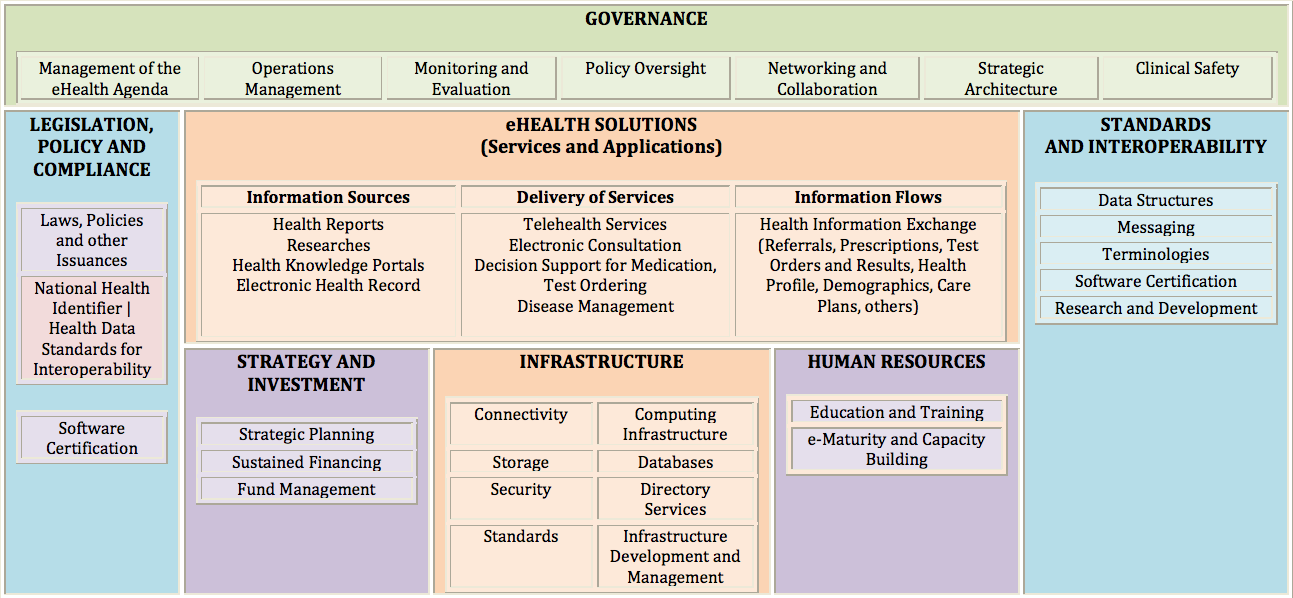
\includegraphics[width=\textwidth]{eHealth}
	\caption{eHealth Component Map from the Philippine eHealth Strategic Framework and Plan 2020 \cite{doh2014ehealth}.}
	\label{fig:eHealth}
\end{figure}